\begin{frame}{Person Re-Identification: Task and Protocol}
  \begin{columns}[T,onlytextwidth]
    \column{0.53\textwidth}
      \begin{itemize}\scriptsize\itemsep0.2em
        \item \textbf{Task.} Person re-identification (re-ID) ranks a gallery of person crops from other cameras so that crops of the query's identity come first. It is retrieval with a learned embedding (query, gallery and mAP as defined earlier in this lecture).
        \item \textbf{Unseen identities.} Training and test identities are disjoint (MSMT17: 1,041 and 3,060), so the embedding must separate people never seen in training. Deciding whether a query matches anyone at all is an open-set problem; open-set recognition is covered later in this lecture.
        \item \textbf{Cross-camera rule.} In the Market-1501 protocol, gallery crops of the query's identity from the query's own camera are ``junk'' and ignored, so every counted match crosses cameras.
        \item \textbf{Cumulative matching characteristic (CMC):} the fraction of queries whose first correct match is in the top $k$,
        \[ \mathrm{CMC}(k) = \frac{1}{|Q|}\sum_{q\in Q}\mathbf{1}\left[\, r_q \leq k \,\right] \]
        $Q$: query set; $r_q$: rank of the first correct gallery crop for $q$; $\mathbf{1}[\cdot]$: 1 if true, else 0. Rank-1 accuracy is $\mathrm{CMC}(1)$.
        \item \textbf{CMC and mAP.} CMC stops at the first hit, yet a Market-1501 query has 14.8 cross-camera ground truths on average, so papers report mAP next to rank-1.
      \end{itemize}
    \column{0.45\textwidth}
      \centering
      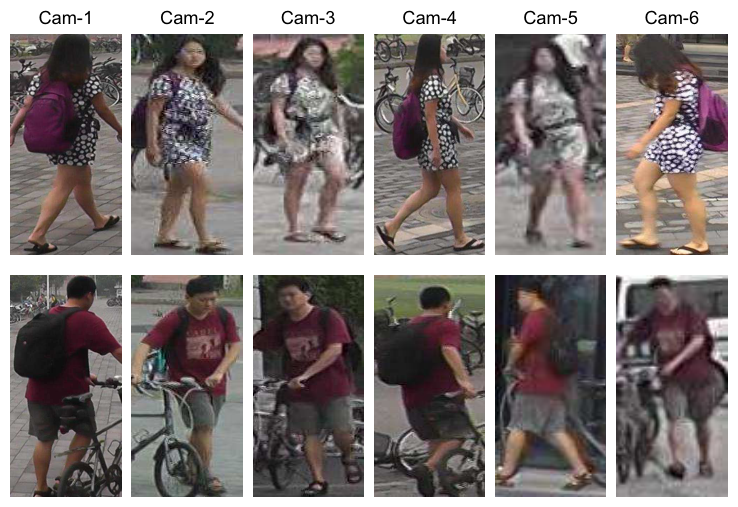
\includegraphics[width=\linewidth,height=0.38\textheight,keepaspectratio]{images/image-recognition/market1501_fig4_queries_six_cameras.png}\\[0.2em]
      {\scriptsize Two identities, one query per camera. Zheng et al., ``Scalable Person Re-Identification: A Benchmark,'' ICCV 2015, \href{https://openaccess.thecvf.com/content_iccv_2015/html/Zheng_Scalable_Person_Re-Identification_ICCV_2015_paper.html}{OpenAccess}, Figure~4.\par}
      \vspace{0.5em}
      {\scriptsize
      \begin{tabular}{lrrr}
        \toprule
        \textbf{Dataset} & \textbf{Identities} & \textbf{Boxes} & \textbf{Cameras} \\
        \midrule
        Market-1501 & 1,501 & 32,668 & 6 \\
        MSMT17 & 4,101 & 126,441 & 15 \\
        \bottomrule
      \end{tabular}\par}
      \vspace{0.2em}
      {\scriptsize MSMT17: multi-scene, multi-time. Counts: Zheng et al., Section~3.1; Wei et al., ``Person Transfer GAN to Bridge Domain Gap for Person Re-Identification,'' CVPR 2018, \href{https://arxiv.org/abs/1711.08565v2}{arXiv:1711.08565v2}, Sections~3.2--3.3.\par}
  \end{columns}
\end{frame}

\begin{frame}{Strong Baseline: ID Loss, Triplet Loss, BNNeck}
  \begin{columns}[T,onlytextwidth]
    \column{0.56\textwidth}
      \begin{itemize}\scriptsize\itemsep0.2em
        \item \textbf{Identity (ID) loss.} Luo et al.\ train ResNet-50 (covered earlier) as an $N$-way classifier over the training identities with softmax cross-entropy (covered earlier) and \textbf{label smoothing}:
        \[ q_i = \begin{cases} 1-\frac{N-1}{N}\,\varepsilon & i = y\\ \varepsilon/N & i \neq y \end{cases} \qquad \mathcal{L}_{\mathrm{ID}} = -\sum_{i=1}^{N} q_i \log p_i \]
        $q_i$: target; $y$: true identity; $p_i$: predicted probability of identity $i$; $\varepsilon = 0.1$. Smoothing curbs overfitting to training identities, which never reappear at test time.
        \item \textbf{Triplet loss} with batch-hard mining (earlier in this lecture): 16 identities $\times$ 4 crops per batch, margin 0.3.
        \item \textbf{BNNeck (batch-norm neck).} ID loss separates identities by angle, triplet loss by Euclidean distance, and on one shared feature the two conflict. BNNeck puts the triplet loss on the pooled feature $f_t$, maps $f_t$ through a batch-norm (BN) layer (covered earlier) to $f_i$, and feeds $f_i$ to a bias-free classifier for the ID loss. Retrieval uses $f_i$ with cosine distance.
        \item \textbf{Last stride 1.} Dropping the downsampling in ResNet-50's last stage turns a $256\times128$ crop into a $16\times8$ feature map, with no new parameters.
        \item \textbf{Market-1501.} Six training tricks, three of them above, lift a standard baseline from 87.7\% rank-1 / 74.0\% mAP to 94.5\% / 85.9\%; BNNeck alone adds 2.1 / 4.0 points.
      \end{itemize}
    \column{0.42\textwidth}
      \centering
      \vspace{1.5em}
      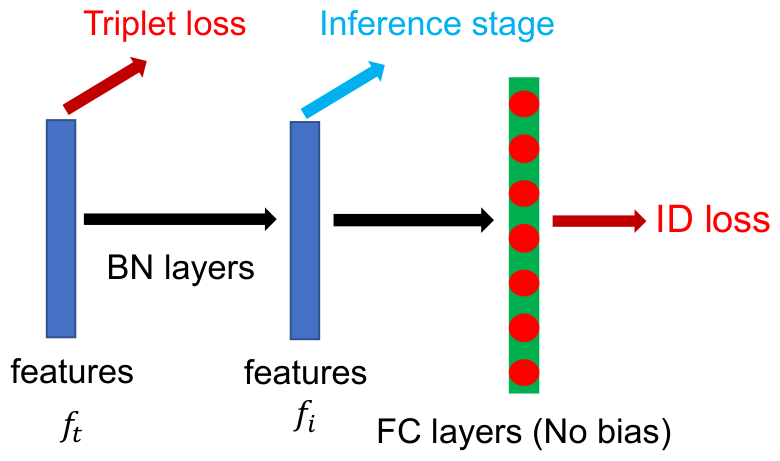
\includegraphics[width=\linewidth,height=0.42\textheight,keepaspectratio]{images/image-recognition/strongbaseline_fig5b_bnneck.png}\\[0.2em]
      {\scriptsize ``In the inference stage, we choose $f_i$ following the BN layer to do the retrieval.'' Luo et al., ``Bag of Tricks and A Strong Baseline for Deep Person Re-identification,'' CVPRW 2019, \href{https://arxiv.org/abs/1903.07071v3}{arXiv:1903.07071v3}, Figure~5(b).\par}
  \end{columns}
\end{frame}

\begin{frame}{TransReID: Side Information and Jigsaw Patches}
  \begin{columns}[T,onlytextwidth]
    \column{0.50\textwidth}
      \begin{itemize}\scriptsize\itemsep0.2em
        \item \textbf{Backbone.} TransReID (He et al., ICCV 2021) swaps the strong baseline's ResNet-50 for ViT-B/16 (covered earlier), with ID and triplet losses on the output class token.
        \item \textbf{Side information embedding (SIE).} A learned vector for the image's camera (and viewpoint, when labelled) is added to every input token:
        \[ Z_0' = Z_0 + \lambda\,\mathcal{S}_C[r] \]
        $Z_0$: patch plus position embeddings; $\mathcal{S}_C[r]$: embedding of camera $r$, shared by all patches of the image; $\lambda$: its weight. The aim is to reduce camera-specific bias.
        \item \textbf{Jigsaw patch module (JPM).} The last transformer layer is split into two independent copies. One outputs the global feature $f_g$; the other shifts and shuffles the patch tokens into $k=4$ groups, and each group plus the class token yields a local feature $f_l^j$ drawn from the whole body. The test feature concatenates $f_g$ and all $f_l^j$.
        \item \textbf{MSMT17 mAP} (Table~5): ViT baseline 61.0, +JPM 63.6, +SIE 62.4, both 64.9. With overlapping patches (sliding window): 67.4 mAP / 85.3 rank-1, and 69.4 / 86.2 at $384\times128$ (Table~6); CNNs in that table reach at most 60.8 mAP.
      \end{itemize}
    \column{0.48\textwidth}
      \centering
      \vspace{1.2em}
      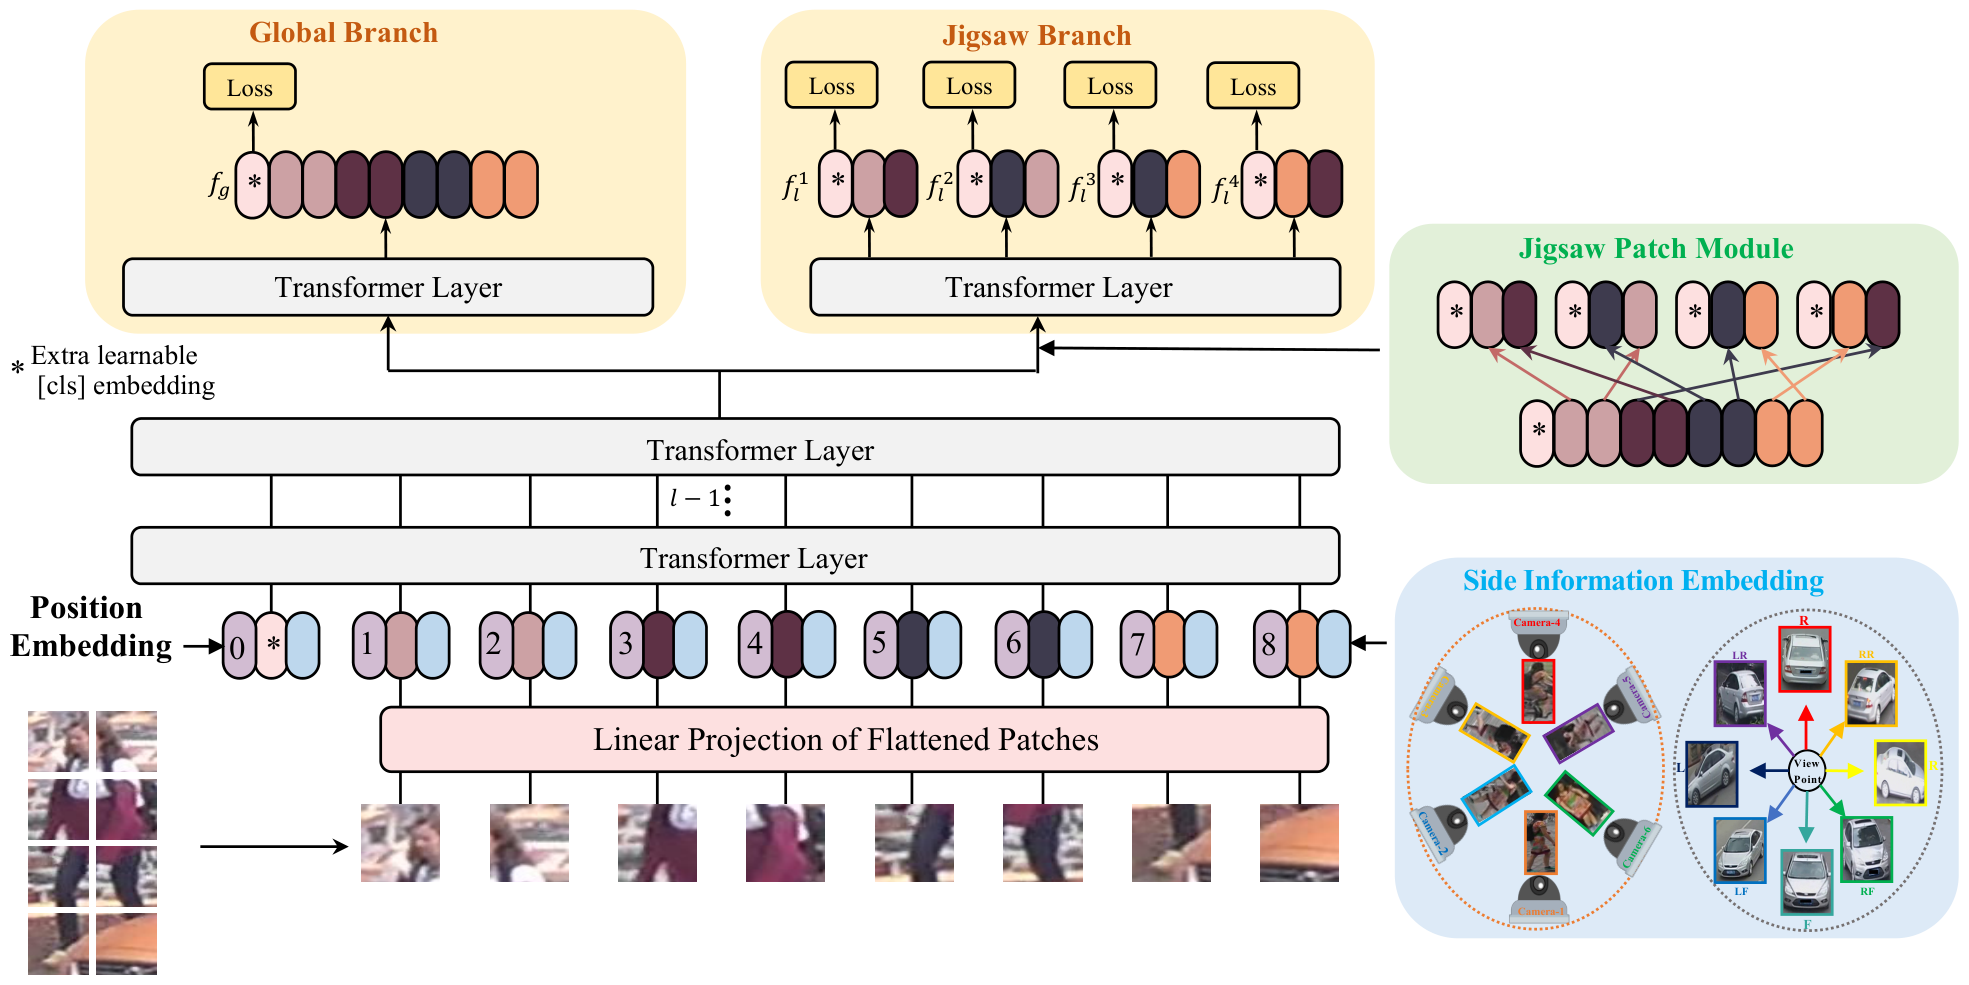
\includegraphics[width=\linewidth,height=0.60\textheight,keepaspectratio]{images/image-recognition/transreid_fig4_framework.png}\\[0.2em]
      {\scriptsize ``Side Information Embedding (light blue) encodes non-visual information such as camera or viewpoint into embedding representations.'' He et al., ``TransReID: Transformer-Based Object Re-Identification,'' ICCV 2021, \href{https://openaccess.thecvf.com/content/ICCV2021/html/He_TransReID_Transformer-Based_Object_Re-Identification_ICCV_2021_paper.html}{OpenAccess}, Figure~4.\par}
  \end{columns}
\end{frame}

\begin{frame}{CLIP-ReID: Learned Text Tokens per Identity}
  \begin{columns}[T,onlytextwidth]
    \column{0.56\textwidth}
      \begin{itemize}\scriptsize\itemsep0.2em
        \item \textbf{The gap.} CLIP (covered earlier) classifies by matching an image to prompts such as ``a photo of a \{label\}''. Re-ID labels are bare indexes, so there is no text to encode.
        \item \textbf{Stage 1.} CLIP-ReID (Li et al., AAAI 2023) gives each training identity $M=4$ learnable tokens in ``A photo of a $[X]_1[X]_2\ldots[X]_M$ person,'' like CoOp's context vectors (earlier in this lecture) but one set per identity. Both CLIP encoders are frozen; only the tokens are trained, with image-to-text and text-to-image contrastive losses in the batch. Each identity $y$ ends with a fixed text feature $T_y$.
        \item \textbf{Stage 2.} With the text side frozen, the image encoder is fine-tuned with ID loss, triplet loss and an image-to-text cross-entropy (i2tce) over all $N$ identities:
        \[ \mathcal{L}_{\mathrm{i2tce}}(i) = -\sum_{k=1}^{N} q_k \log \frac{\exp\big(s(V_i, T_{y_k})\big)}{\sum_{a=1}^{N} \exp\big(s(V_i, T_{y_a})\big)} \]
        $V_i$: feature of image $i$; $s$: dot product of projected features; $q_k$: label-smoothed target. The $T_y$ act as fixed class prototypes.
        \item \textbf{MSMT17, ViT-B/16} (Tables~2 and 5): CLIP's image encoder with the usual re-ID losses, 66.1 mAP; tokens and encoder trained together in one stage, 68.9; two stages, 73.4 mAP / 88.7 rank-1, or 75.8 / 89.7 with SIE and overlapping patches (TransReID with both: 67.4 / 85.3). Market-1501: 89.6 / 95.5.
      \end{itemize}
    \column{0.42\textwidth}
      \centering
      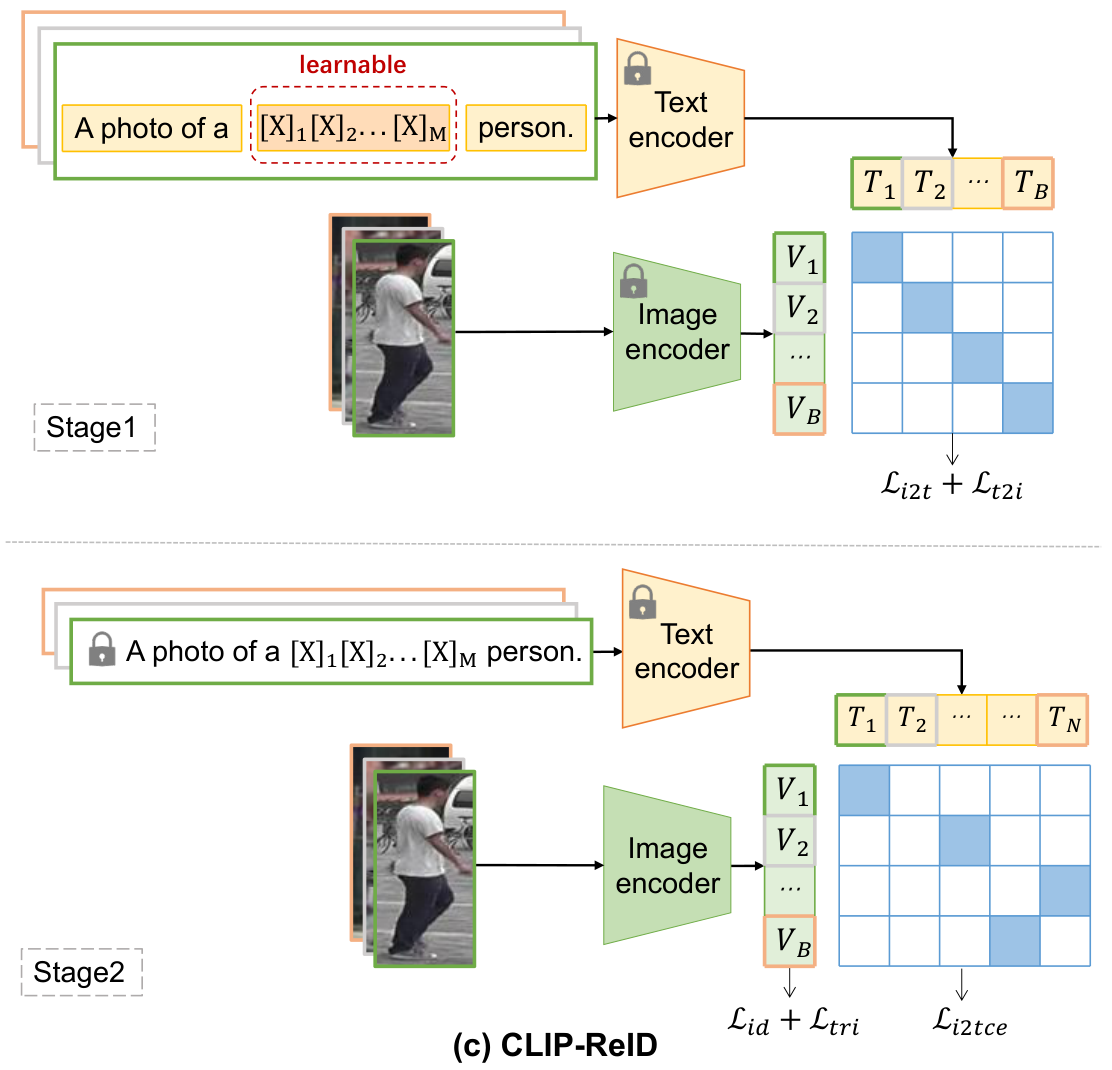
\includegraphics[width=\linewidth,height=0.62\textheight,keepaspectratio]{images/image-recognition/clipreid_fig2c_two_stage_training.png}\\[0.2em]
      {\scriptsize Locks mark frozen parts. Li et al., ``CLIP-ReID: Exploiting Vision-Language Model for Image Re-Identification without Concrete Text Labels,'' AAAI 2023, \href{https://arxiv.org/abs/2211.13977v4}{arXiv:2211.13977v4}, Figure~2(c).\par}
  \end{columns}
\end{frame}

\begin{frame}{Pretraining on People: LUPerson and SOLIDER}
  \begin{columns}[T,onlytextwidth]
    \column{0.52\textwidth}
      \begin{itemize}\scriptsize\itemsep0.2em
        \item \textbf{LUPerson} (Fu et al., CVPR 2021): 4,180,243 unlabelled person crops detected in YouTube street-view videos, from an estimated 219,848 people. Contrastive pretraining on it with MoCo v2 (MoCo covered earlier) shows colour jitter to be harmful, since colour is a main cue for telling people apart.
        \item \textbf{SOLIDER} (semantic controllable self-supervised learning; Chen et al., CVPR 2023) starts from DINO (covered earlier), whose features group a person's parts by appearance. It clusters token features with k-means (covered earlier) into background and three parts ordered top to bottom (upper body, lower body, shoes) and adds a token-level classification loss on these pseudo-labels.
        \item \textbf{Semantic controller.} A scalar $\lambda\in[0,1]$ becomes a scale and a shift on the features after every Swin block (covered earlier) and weights the part loss:
        \[ \mathcal{L} = \alpha\,\mathcal{L}_{\mathrm{dino}}\big(F(\lambda)\big) + \lambda\,(1-\alpha)\,\mathcal{L}_{\mathrm{sm}}\big(F(\lambda)\big) \]
        $F(\lambda)$: features under $\lambda$; $\mathcal{L}_{\mathrm{dino}}$: DINO loss; $\mathcal{L}_{\mathrm{sm}}$: part loss; $\alpha=0.5$. Re-ID fine-tunes with $\lambda$ = 0.0--0.2 (appearance), parsing and detection with 0.8--1.0.
      \end{itemize}
    \column{0.46\textwidth}
      \centering
      {\scriptsize Fine-tuned with TransReID on Swin-T (tiny), mAP / rank-1:\par}
      \vspace{0.3em}
      {\scriptsize
      \begin{tabular}{lcc}
        \toprule
        \textbf{Pretraining} & \textbf{MSMT17} & \textbf{Market-1501} \\
        \midrule
        ImageNet, supervised & 49.7 / 73.6 & 78.1 / 90.2 \\
        LUP1M, DINO & 63.3 / 83.2 & 89.6 / 95.9 \\
        \quad + part labels & 61.6 / 82.2 & 89.5 / 95.5 \\
        \quad + controller & 63.9 / 83.8 & 89.9 / 96.1 \\
        \bottomrule
      \end{tabular}\par}
      \vspace{0.2em}
      {\scriptsize Last row: SOLIDER. LUP1M: a random 1M-image subset of LUPerson, close to ImageNet in size. Chen et al., ``Beyond Appearance: a Semantic Controllable Self-Supervised Learning Framework for Human-Centric Visual Tasks,'' CVPR 2023, \href{https://arxiv.org/abs/2303.17602v1}{arXiv:2303.17602v1}, Table~1.\par}
      \begin{itemize}\scriptsize\itemsep0.2em
        \item Self-supervised pretraining on person crops instead of supervised ImageNet adds 13.6 mAP on MSMT17; the authors credit LUPerson's street scenes, which resemble re-ID data. Part labels alone cost 1.7 mAP; with the controller, SOLIDER ends 0.6 above plain DINO.
        \item SOLIDER on Swin-B (base): 77.1 mAP / 90.7 rank-1 on MSMT17, 93.9 / 96.9 on Market-1501 (Table~2).
      \end{itemize}
  \end{columns}
\end{frame}

\begin{frame}{Re-ID Beyond the Standard Benchmark}
  \begin{columns}[T,onlytextwidth]
    \column{0.52\textwidth}
      \begin{itemize}\scriptsize\itemsep0.3em
        \item \textbf{Clothes-changing re-ID.} Most re-ID work assumes people keep their clothes, and models overfit to clothing. The clothes-based adversarial loss (CAL; Gu et al., CVPR 2022) alternates, on colour (RGB) images only: fit a clothes classifier on the backbone features, then train the backbone so that this classifier cannot tell one identity's outfits apart. On the PRCC benchmark CAL reaches 100\% rank-1 with the same clothes and 55.2\% with changed clothes (Table~2).
        \item \textbf{Animal re-ID.} Ecologists identify individual animals from markings. MegaDescriptor (Cermak et al., WACV 2024) is a Swin-L (large) trained with ArcFace (earlier in this lecture) on 29 public animal datasets; a query takes the identity of its nearest reference image by cosine similarity, and every query animal is in the reference set. On the HumpbackWhaleID dataset, whose reference images were part of its training data, it is right for 77.81\% of queries, off-the-shelf DINOv2 (ViT-L) features for 6.44\% (Table~4).
        \item \textbf{Instruction-driven re-ID.} Instruct-ReID (He et al., CVPR 2024) handles six re-ID variants as one task by attaching an instruction to the query: a phrase such as ``Ignore clothes'', a clothing image, or sentences describing the target. With sentences (COCAS+ Real2 test set), mAP goes from 14.9 for a ViT-B that ignores the text to 39.8 for their multi-task model (Table~4).
      \end{itemize}
    \column{0.46\textwidth}
      \centering
      \vspace{0.8em}
      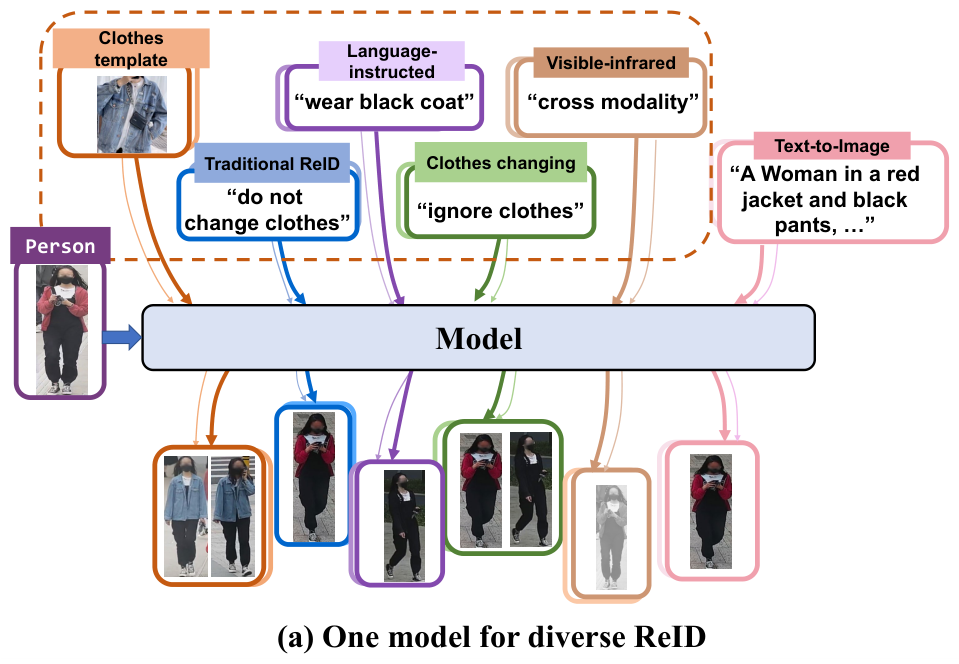
\includegraphics[width=\linewidth,height=0.60\textheight,keepaspectratio]{images/image-recognition/instructreid_fig1a_one_model_many_tasks.png}\\[0.2em]
      {\scriptsize Six re-ID tasks expressed as instructions to one model. He et al., ``Instruct-ReID: A Multi-purpose Person Re-identification Task with Instructions,'' CVPR 2024, \href{https://openaccess.thecvf.com/content/CVPR2024/html/He_Instruct-ReID_A_Multi-purpose_Person_Re-identification_Task_with_Instructions_CVPR_2024_paper.html}{OpenAccess}, Figure~1(a).\par}
  \end{columns}
\end{frame}

\begin{frame}{Re-ID and Privacy: Engineering Practice}
  \begin{itemize}\scriptsize\itemsep0.25em
    \item \textbf{A surveillance technology.} Re-ID ``aims to search the target person from surveillance videos across different locations and times'' (Gu et al., CVPR 2022). Matches across cameras and hours add up to a record of where a person went, and errors are routine: SOLIDER's 90.7\% rank-1 on MSMT17 still ranks a different person first for 9.3\% of queries.
    \item \textbf{Data with a history.} DukeMTMC, the multi-camera tracking dataset from which the DukeMTMC-reID benchmark was cut, was retracted by its creators in April 2019 after an investigation raised ethical concerns about how the data was collected and used. Copies kept circulating through derived datasets: a 20\% sample of citing papers contains 73 uses in 2020. LUPerson was cut from crawled YouTube videos, and its paper describes no consent or face-blurring step.
  \end{itemize}
  \vspace{0.2em}
  {\centering\scriptsize
  \begin{tabular}{p{2.9cm} p{9.5cm}}
    \toprule
    \textbf{Practice} & \textbf{What it means for a re-ID system} \\
    \midrule
    Decide whether to build it & State who is searched, by whom, and what follows a match; stop if the answer is open-ended tracking of people. \\
    Fixed scope & Fix the task, the cameras and the time window; reject queries outside them. \\
    Access control & Restrict who can query; log every query with its reason, and review the log. \\
    Deletion schedule & Delete crops and embeddings after a fixed period; keep only needed aggregates. \\
    Opt-in where possible & Prefer settings where people agree to take part (a team studying its own players) and wildlife. \\
    Human review & No automatic action on a match; a person checks each result first. \\
    Dataset stewardship & Terms of use that cover trained models and derivatives; retraction notices on all copies. \\
    \bottomrule
  \end{tabular}\par}
  \vspace{0.1em}
  {\scriptsize Retraction facts and the stewardship row: Peng et al., ``Mitigating Dataset Harms Requires Stewardship: Lessons from 1000 Papers,'' NeurIPS 2021 Datasets and Benchmarks Track, \href{https://arxiv.org/abs/2108.02922v2}{arXiv:2108.02922v2}, Figure~1, Table~2 and Section~8.1. The other rows are course guidance.\par}
\end{frame}
